% ARTICLE 2 ----
% This is just here so I know exactly what I'm looking at in Rstudio when messing with stuff.
% Options for packages loaded elsewhere
\PassOptionsToPackage{unicode}{hyperref}
\PassOptionsToPackage{hyphens}{url}
%
\documentclass[
  11pt,
]{article}
\usepackage{lmodern}
\usepackage{amssymb,amsmath}
\usepackage{ifxetex,ifluatex}
\ifnum 0\ifxetex 1\fi\ifluatex 1\fi=0 % if pdftex
  \usepackage[T1]{fontenc}
  \usepackage[utf8]{inputenc}
  \usepackage{textcomp} % provide euro and other symbols
\else % if luatex or xetex
  \usepackage{unicode-math}
  \defaultfontfeatures{Scale=MatchLowercase}
  \defaultfontfeatures[\rmfamily]{Ligatures=TeX,Scale=1}
\fi
% Use upquote if available, for straight quotes in verbatim environments
\IfFileExists{upquote.sty}{\usepackage{upquote}}{}
\IfFileExists{microtype.sty}{% use microtype if available
  \usepackage[]{microtype}
  \UseMicrotypeSet[protrusion]{basicmath} % disable protrusion for tt fonts
}{}
\makeatletter
\@ifundefined{KOMAClassName}{% if non-KOMA class
  \IfFileExists{parskip.sty}{%
    \usepackage{parskip}
  }{% else
    \setlength{\parindent}{0pt}
    \setlength{\parskip}{6pt plus 2pt minus 1pt}
    }
}{% if KOMA class
  \KOMAoptions{parskip=half}}
\makeatother
\usepackage{xcolor}
\IfFileExists{xurl.sty}{\usepackage{xurl}}{} % add URL line breaks if available
\urlstyle{same} % disable monospaced font for URLs
\usepackage[margin=1in]{geometry}
\usepackage{graphicx}
\makeatletter
\def\maxwidth{\ifdim\Gin@nat@width>\linewidth\linewidth\else\Gin@nat@width\fi}
\def\maxheight{\ifdim\Gin@nat@height>\textheight\textheight\else\Gin@nat@height\fi}
\makeatother
% Scale images if necessary, so that they will not overflow the page
% margins by default, and it is still possible to overwrite the defaults
% using explicit options in \includegraphics[width, height, ...]{}
\setkeys{Gin}{width=\maxwidth,height=\maxheight,keepaspectratio}
% Set default figure placement to htbp
\makeatletter
\def\fps@figure{htbp}
\makeatother
\setlength{\emergencystretch}{3em} % prevent overfull lines
\providecommand{\tightlist}{%
  \setlength{\itemsep}{0pt}\setlength{\parskip}{0pt}}
\setcounter{secnumdepth}{5}

\ifluatex
  \usepackage{selnolig}  % disable illegal ligatures
\fi


\title{Appendix of: Why and when do (Czech) judges dissent: an empirical
analysis of the Czech Constitutional Court}
\author{true \and true}
\date{August 31, 2023}

% Jesus, okay, everything above this comment is default Pandoc LaTeX template. -----
% ----------------------------------------------------------------------------------
% I think I had assumed beamer and LaTex were somehow different templates.


\usepackage{kantlipsum}

\usepackage{abstract}
\renewcommand{\abstractname}{}    % clear the title
\renewcommand{\absnamepos}{empty} % originally center

\renewenvironment{abstract}
 {{%
    \setlength{\leftmargin}{0mm}
    \setlength{\rightmargin}{\leftmargin}%
  }%
  \relax}
 {\endlist}

\makeatletter
\def\@maketitle{%
  \newpage
%  \null
%  \vskip 2em%
%  \begin{center}%
  \let \footnote \thanks
      {\fontsize{18}{20}\selectfont\raggedright  \setlength{\parindent}{0pt} \@title \par}
    }
%\fi
\makeatother


\title{Appendix of: Why and when do (Czech) judges dissent: an empirical
analysis of the Czech Constitutional Court }

\date{}

\usepackage{titlesec}

% 
\titleformat*{\section}{\large\bfseries}
\titleformat*{\subsection}{\normalsize\itshape} % \small\uppercase
\titleformat*{\subsubsection}{\normalsize\itshape}
\titleformat*{\paragraph}{\normalsize\itshape}
\titleformat*{\subparagraph}{\normalsize\itshape}

% add some other packages ----------

% \usepackage{multicol}
% This should regulate where figures float
% See: https://tex.stackexchange.com/questions/2275/keeping-tables-figures-close-to-where-they-are-mentioned
\usepackage[section]{placeins}



\makeatletter
\@ifpackageloaded{hyperref}{}{%
\ifxetex
  \PassOptionsToPackage{hyphens}{url}\usepackage[setpagesize=false, % page size defined by xetex
              unicode=false, % unicode breaks when used with xetex
              xetex]{hyperref}
\else
  \PassOptionsToPackage{hyphens}{url}\usepackage[draft,unicode=true]{hyperref}
\fi
}

\@ifpackageloaded{color}{
    \PassOptionsToPackage{usenames,dvipsnames}{color}
}{%
    \usepackage[usenames,dvipsnames]{color}
}
\makeatother
\hypersetup{breaklinks=true,
            bookmarks=true,
            pdfauthor={Štěpán Paulík (Humboldt Universität zu Berlin,
\href{mailto:stepan.paulik.1@hu-berlin.de}{\nolinkurl{stepan.paulik.1@hu-berlin.de}}) and Gor
Vartazaryan (Charles University,
\href{mailto:gorike2000@gmail.com}{\nolinkurl{gorike2000@gmail.com}})},
             pdfkeywords = {},
            pdftitle={Appendix of: Why and when do (Czech) judges
dissent: an empirical analysis of the Czech Constitutional Court},
            colorlinks=true,
            citecolor=blue,
            urlcolor=blue,
            linkcolor=magenta,
            pdfborder={0 0 0}}
\urlstyle{same}  % don't use monospace font for urls

% Add an option for endnotes. -----



% This will better treat References as a section when using natbib
% https://tex.stackexchange.com/questions/49962/bibliography-title-fontsize-problem-with-bibtex-and-the-natbib-package

% set default figure placement to htbp
\makeatletter
\def\fps@figure{htbp}
\makeatother



\usepackage{longtable}
\LTcapwidth=.95\textwidth
\linespread{1.05}
\usepackage{hyperref}
\usepackage{float}

\newtheorem{hypothesis}{Hypothesis}

\usepackage{setspace}

% trick for moving figures to back of document
% really wish we'd knock this shit off with moving tables/figures to back of document
% but, alas...

% 
% Optional code chunks ------
% SOURCE: https://stackoverflow.com/questions/50702942/does-rmarkdown-allow-captions-and-references-for-code-chunks



\begin{document}

% \textsf{\textbf{This is sans-serif bold text.}}
% \textbf{\textsf{This is bold sans-serif text.}}


% \maketitle

{% \usefont{T1}{pnc}{m}{n}
\setlength{\parindent}{0pt}
\thispagestyle{plain}
{%\fontsize{18}{20}\selectfont\raggedright
\maketitle  % title \par

}




{
   \vskip 13.5pt\relax \normalsize\fontsize{11}{12}
   \MakeUppercase{Štěpán Paulík}, \small{Humboldt Universität zu Berlin,
\href{mailto:stepan.paulik.1@hu-berlin.de}{\nolinkurl{stepan.paulik.1@hu-berlin.de}}}   \par \vskip -3.5pt \MakeUppercase{Gor
Vartazaryan}, \small{Charles University,
\href{mailto:gorike2000@gmail.com}{\nolinkurl{gorike2000@gmail.com}}}   

}

}






\vskip -8.5pt

{
\hypersetup{linkcolor=black}
\setcounter{tocdepth}{2}
\tableofcontents
}

 % removetitleabstract

{
\setcounter{tocdepth}{2}
\tableofcontents
}

\setlength{\parindent}{16pt}
\setlength{\parskip}{0pt}

% We'll put doublespacing here
\doublespacing
% Remember to cut it out later before bib
\vspace{30pt}

This is an appendix, in which we diagnose and compare the models from
our main article and explain our choices in higher detail.

\hypertarget{model-1-effect-of-presence-of-dissenting-opinion-on-the-length-of-majority-argumentation}{%
\section{Model 1: Effect of presence of dissenting opinion on the length
of majority
argumentation}\label{model-1-effect-of-presence-of-dissenting-opinion-on-the-length-of-majority-argumentation}}

\hypertarget{caselaw-partitioning-classification}{%
\subsection{Caselaw partitioning
classification}\label{caselaw-partitioning-classification}}

\hypertarget{statistical-model}{%
\subsection{Statistical model}\label{statistical-model}}

\hypertarget{model-specification}{%
\subsubsection{Model specification}\label{model-specification}}

We opted for a completely pooled model as the data did not contain any
inherent structure (there were no clusters). At first glance, we assumed
that

\[
Y | \lambda \sim Pois(\lambda)
\]

because our outcome variable of interest is a discrete count and the
density plot of the length of court argumentation suggests so.

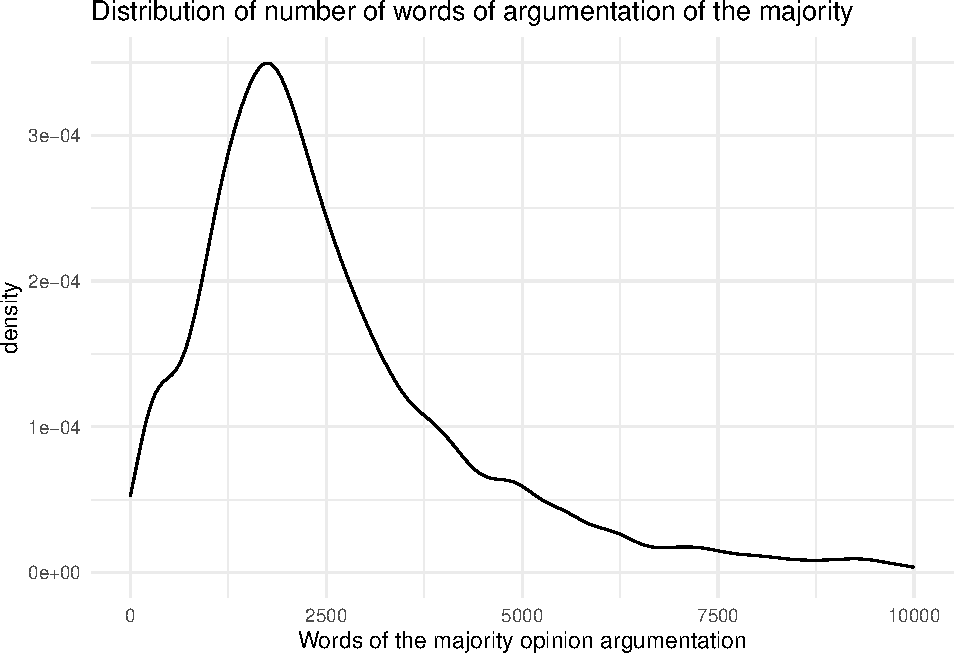
\includegraphics{dissents_article_appendix_files/figure-latex/negbinom-1.pdf}

However, as the posterior checking revealed, the Y was actually
overdispersed and the Poisson regression was not able to capture the
overdispersion. Therefore, we instead opted for the Negative Binomial
model, which allows for relaxing the assumption of equality of variance
of Y to its expected value. Thus, the explanatory variable, the number
of words of argumentation of the CCC \emph{Y}

\[
Y_{words} | \mu, r \sim NegBin(\mu, r)
\]

As for the priors, we based the priors on the Epstein results as well as
a cursory exploratory peak into the data. All our priors follow a normal
distribution, the intercept being centered around the population mean.
The remaining priors were kept uninformative, because we simply have no
previous knowledge on the CCC.

\hypertarget{model-diagnosis}{%
\subsubsection{Model diagnosis}\label{model-diagnosis}}

We ran the model via Stan with 4 Monte Carlo Markov Chains (MCMC) of
20000 iterations each, the first 10000 warm up iterations being
discarded. The trace plot shows that the chains were stable and probed
plausible parameter values, the density plots of the MCMC show that all
4 chains exhibited similar behavior, and the autocorrelation between the
iterations always dropped quickly and that the chains were moving around
the potential parameter values quickly.

The posterior diagnosis confirms that although the simulations are not
perfect, they do reasonably capture the features of the observed number
of words of court arguments. In other words, we selected the correct
model and the priors are not too off either. Thus, our Negative Binomial
regression assumptions are reasonable.

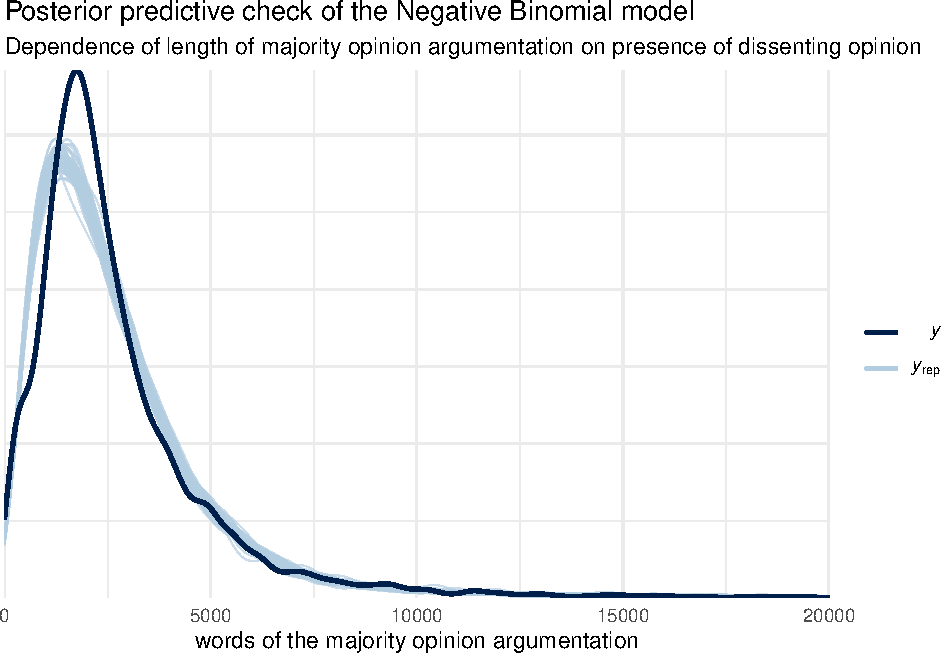
\includegraphics{dissents_article_appendix_files/figure-latex/pp_check_negbinom-1.pdf}

\hypertarget{model-2-effect-of-workload-on-the-dissenting-behavior}{%
\section{Model 2: Effect of workload on the dissenting
behavior}\label{model-2-effect-of-workload-on-the-dissenting-behavior}}

\hypertarget{model-diagnosis-1}{%
\subsection{Model diagnosis}\label{model-diagnosis-1}}

We tried two models, a completely pooled and hierarchical model
clustered around the judges. The main difference between the two models
is that the former model completely ignores individual intercept. The
latter allows for differentiating intercepts between the groups (in our
case the individual judges) and the global intercept. The global
parameter of interest is then informed both by the global trends as well
as the individual intercepts. That can usually lead to higher accuracy
in case of structured or time series data at the cost of higher
computational expenses.

We ran both the models via Stan with 4 Monte Carlo Markov Chains (MCMC)
of 20000 iterations each, the first 10000 warm up iterations being
discarded. We did a diagnosis of all the models. In all cases, the trace
plots show that the chains were stable and probed plausible parameter
values, the density plots of the MCMC show that all 4 chains exhibited
similar behavior, and the autocorrelation between the iterations always
dropped quickly and that the chains were moving around the potential
parameter values quickly.

We now compare the pooled against the hierarchical models. The former
model got the posterior prediction 1.2 of the number of dissents per
judge wrong (0.84 standard deviations off), whereas the former model got
the posterior prediction wrong only by 0.94 of the number of dissents
per judge (0.7 standard deviations off), with 99 \% of the predictions
falling within the 95 \% posterior credible interval. 6-fold
cross-validated check reveals that neither of the models overfitted.
Thus, while the hierarchical model is slightly more computationally
expensive, it yields better results. \# Model 3: Collegiality costs of
dissenting at the CCC \#\# Model diagnosis We ran the model via Stan
with 4 Monte Carlo Markov Chains (MCMC) of 20000 iterations each, the
first 10000 warm up iterations being discarded. We did diagnosis of all
the models. The trace plots reveal that the chains were stable and
probed plausible parameter values, the density plots of the MCMC show
that all 4 chains exhibited similar behavior, and the autocorrelation
between the iterations always dropped quickly and that the chains were
moving around the potential parameter values quickly.The posterior
predictive check again reveals that our posterior model reasonably
captures the underlying data.

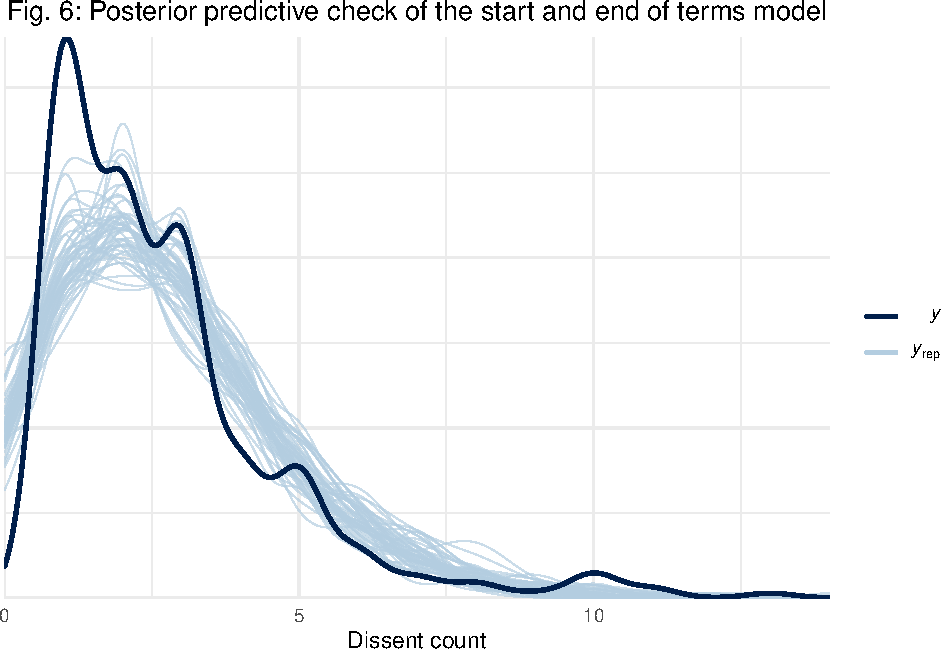
\includegraphics{dissents_article_appendix_files/figure-latex/posterior_check_term-1.pdf}

\end{document}
